\documentclass{article}
\usepackage[utf8]{inputenc}
\usepackage[T1]{fontenc}
\usepackage{array}
\usepackage{tabu}
\usepackage{hyperref}
\usepackage{longtable}
\usepackage{graphicx}
\graphicspath{ {use_cases/} }
\newcommand{\breakline}{\rule{\linewidth}{0.5mm}}


\title{
{
    
\includegraphics[width=0.25\textwidth]{SRS/slike/logo.png}~\\[0.1cm]
    \textsc{\Large Univerzitet u Sarajevu}\\[0.2cm]  
    \textsc{\Large Elektrotehnički fakultet} \\[0.5cm] 
    \huge \bfseries BulletinBoard} \\[0.4cm] 
    \breakline \\[0.5cm]
    \textsc{\Large Software Requirements Specification}\\[0.4cm]
    }
    
\author{\begin{tabular}{rl}
  \textbf{Mentori:} & R. prof. dr Novica Nosović, dipl.ing.el.e \\ &
                    Haseljić Hana, MoE \\
  \textbf{Članovi tima:} & Građanin Ehvan \\ 
                        & Hadžihasanović Lamija \\ 
                        & Hadžirović Kenan \\ 
                        & Hajdarević Ena \\ 
                        & Halilović Haris \\ 
                        & Halilović Irhad \\ 
                        & Haseljić Emira
\end{tabular}}

\date{\textbf{Akademska 2017/2018}}

\begin{document}
\maketitle
\newpage
\renewcommand{\contentsname}{Sadržaj}
\tableofcontents
\newpage

\section*{Historijat revizije dokumenta}


\begin{center}
\begin{tabular}{ |c |c |c |c|} \hline
 Datum & Verzija & Autor & Komentar\\ \hline
 13.4.2018. & v1.1 & PinboardTeam  & Ispravljene greške i dodan korisnički interfejs. \\  \hline
 28.3.2018. & v1.0 & PinboardTeam  & Prva verzija dokumenta. \\  \hline
\end{tabular}
\end{center}
\newpage


\section{Uvod}
\subsection{Svrha dokumenta}
Ovaj dokument je osnovna referenca za opis softverskog proizvoda BulletinBoard. Sadrži informacije o zahtjevima i karakteristikama koje opisuju dati softverski sistem.

Kroz poglavlja ovog dokumenta opisani su namjena softverskog sistema, načini korištenja kao i uslovi koji moraju biti zadovoljeni da bi on ispravno funkcionisao. 
Funkcionalni i nefunkcionalni zahtjevi postavljeni pred sistem, kao i načini na koje su oni zadovoljeni su pobrojani kao važan dio dokumentovanja sistema.
Korisnik treba da stekne jasnu sliku o načinu korištenja softvera, kao i osnovno znanje o mogućim postupcima prilikom otklanjanja grešaka u radu. Razvojni tim koristi dokument kao referencu za zahtjeve i ograničenja postavljena pred njih.
\subsection{Opseg (scope) dokumenta}
Dokument služi razvojnom timu i korisnicima sistema kako bi stekli sliku o namjeni i funkcionalnostima prozivoda. To se postiže detaljnim opisivanjem načina korištenja, funkcionalnih zahtjeva koji se postavljaju pred proizvod kao i nefunkcionalnih zahtjeva i ograničenja. 

Proizvod je namjenjen širokoj publici korisnika tako da koristi vokabular razumljiv svima. Rječnik tehničkih pojmova je priložen na početku dokumenta kao referenca za bolje razumjevanje.

Koriste se UML dijagrami za opis osnovnih funkcionalnosti, procesa i aktivnosti unutar sistema. Oni pružaju općenitu sliku dešavanja u sistemu, ne ulazeći u implementacione detalje pojedinačnih funkcionalnosti.

Obzirom da dokumentacija u svakom trenutku treba ispravno opisivati sistem o kojem piše, dokument može doživljavati eventualne izmjene u skladu sa promjenama zahtjeva ili osobina softvera. Te promjene su zabilježene na početku dokumenta u poglavlju Historijat revizije dokumenta.
\newpage
\subsection{Definicije, akronimi i kratice}

\begin{center}
    \begin{longtable}{|c |m{8cm} |} \hline
        \textbf{Pojam} & \textbf{Opis} \\ \hline
        \textbf{API} & Application Programming Interface, pristupna tačka softverskog sistema pomoću koje sistem razmjenjuje podatke sa drugim sistemima ili korisnicima. \\  \hline
        \textbf{Aplikacija} & Računarski program namnjenjen izvršavanju jednog ili više korisničkih zahtjeva. \\ \hline
        \textbf{Cloud} & Korištenje resursa iznajmljenih od drugih kompanija ili organizacija za potrebe hostinga aplikacija, spremanja podataka i sličnih internet usluga. \\ \hline
        \textbf{ERD} & Entity Relationship Diagram, dijagram koji opisuje strukturu baze podataka određenog sistema. \\  \hline
        \textbf{Funkcionalni zahtjev} & Opis servisa koje sistem nudi, ponašanje sistema na određene ulaze i u određenim situacijama.\\ \hline
        \textbf{Hosting} & Usluga koja omogućava pristup web stranicama ili aplikacijama putem internet veze. Kompanije vlasnici serverskih mašina iznajmljuju mašine ili njihove dijelove krajnjem klijentu za potrebe informacionog sistema. \\ \hline
        \textbf{HTTP} & Hypertext Transfer Protocol je aplikacioni protokol koji služi za prenos podataka na world wide webu. \\  \hline
        \textbf{IEEE} & Institute of Electrical and Electronics Engineers, svjetski institut (udruženje) inženjera elektrotehnike. Zaslužan za standardizaciju u mnogim poljima informatike i elektrotehnike. \\  \hline
        \textbf{IEEE 830-1998 Standard} & Set preporučenih praksi za definisanje SRS (Software Requirements Specification) dokumenta kao osnovne dokumentacije softverskog sistema. \\  \hline
        \textbf{ISP} & Internet Service Provider, pružalac usluge konekcije na internet. Iznajmljuje uslugu pristupa, kao i potrebni hardver i softver za korištenje interneta. \\ \hline
        \textbf{Nefunkcionalni zahtjev} & Ograničenja na servise koje sistem nudi u zavisnosti od vremena, okolnosti, razvojnog procesa, standarda i sl. \\ \hline
        \textbf{Operativni sistem} & Sistemski softver koji upravlja komunikacijom između softvera i hardvera. \\ \hline
        \textbf{Provider} & Pružalac određene usluge. (npr. Internet Service Provider) \\ \hline
        \textbf{Server} & Računar koji pruža uslugu drugim, klijentskim računarima.  \\ \hline
        \textbf{SLA} & Service Level Agreement je ugovor kojim se definiše vrsta i nivo usluge između klijenta i onog ko mu nudi uslugu (servis provajdera). \\ \hline
        \textbf{SRS} & Software Requirements Specification je osnovni dio dokumentovanja softverskog sistema. Sadrži funkcionalne i nefunkcionalne zahtjeve, dijagrame aktivnosti i načina korištenja, te interakcije unutar sistema. Konačno, SRS definira i interfejse pomoću kojih sistem komunicira sa vanjskim svjetom, konkretno sa drugim korisnicima i sistemima.\\ \hline
        \textbf{Tooltip} & Pomoćni tekst iznad komponenti grafičkog interfejsa koji služi da pojasni funkcionalnost ili njen status. \\  \hline
        \textbf{UML} & Unified Modeling Language je grafički jezik za vizualiziranje, specificiranje, konstruiranje i dokumentiranje sistema programske podrške prema definiciji OMG (Object Management Group) grupe. \\  \hline
        \textbf{Web Aplikacija} & Aplikacija koja se izvršava u web pregledniku korisničkog računara. \\ \hline
        \textbf{Web Preglednik} & Aplikativni softver koji omogućava pretraživanje world wide weba. \\ \hline
    \end{longtable}
\end{center}
\newpage
\subsection{Standardi dokumentovanja}
Dokument je pisan u skladu sa IEEE 830-1988 standardom.
Dokument je pisan u Latex sistemu za pripremu dokumenata.
Autori dokumenta su članovi tima SI Pinboard Team.
\subsection{Reference}
\begin{itemize}
  \item IEEE 830 - 1998 Standard -  \url{https://github.com/SoftverInzenjeringETFSA/2018_BulletinBoard/raw/master/Dokumentacija/Reference/IEEE830.pdf}
\end{itemize}

\newpage
\section{Opis}
\subsection{Perspektiva proizvoda}
Bulletinboard je samostalna web aplikacija koja sadrži svoju bazu smještenu na odvojenom računaru (serveru) i za pristup aplikaciji je neophodna Internet konekcija.
\subsection{Funkcionalnosti proizvoda}
\subsubsection{Bulletinboard profil}
Bulletinboard profil omogučava sljedeče pogodnosti:
\begin{itemize}
    \item Odličan način praćenja personalnog progresa
    \item Efektivno organizovanje vremena i taskova
    \item Mjesto za pregled odabranih sadržaja
    \item Mjesto za efektivno informisanje
    \item Brzo dijeljenje potrebnog sadržaja sa društvenih mreža
    \item Poticanje inspiracije, efikasnosti i kreativnosti
    \item Povećava interesovanje i motivaciju
    \item Kalendarsku organizaciju vremena
\end{itemize}

\subsubsection{Administracija korisnika}
Upravljanje klijentima zahtijeva privilegovani pristup administratora, a uključuje:
\begin{itemize}
    \item Kreiranje novog korisnika
    \item Modifikacija postojećeg korisnika
    \item Brisanje postojećeg korisnika
    \item Opcija ban-ovanja (zabrana pristupa korisniku)
    \item Pretraga i pregled korisnika
\end{itemize}

\subsection{Karakteristike korisnika}
Svi korisnici imaju iste mogućnosti upotrebe aplikacije. Izdvajaju se administratori sistema koji su zaduženi za održavanje korisničkih računa.
\subsubsection{Mogućnosti korisnika}
Korisnik sistema ima sljedeće mogućnosti:
\begin{itemize}
    \item Prijava na sistem
    \item Odjava sa sistema
    \item Kreiranje neovog korisničkog računa
    \item Dodavanje slike
    \item Brisanje slike
    \item Dijeljenje sadržaja sa društvenih mreža
    \item Dodavanje posta
    \item Brisanje posta
    \item Dodavanje posta sa datumom(kalendar)
\end{itemize}
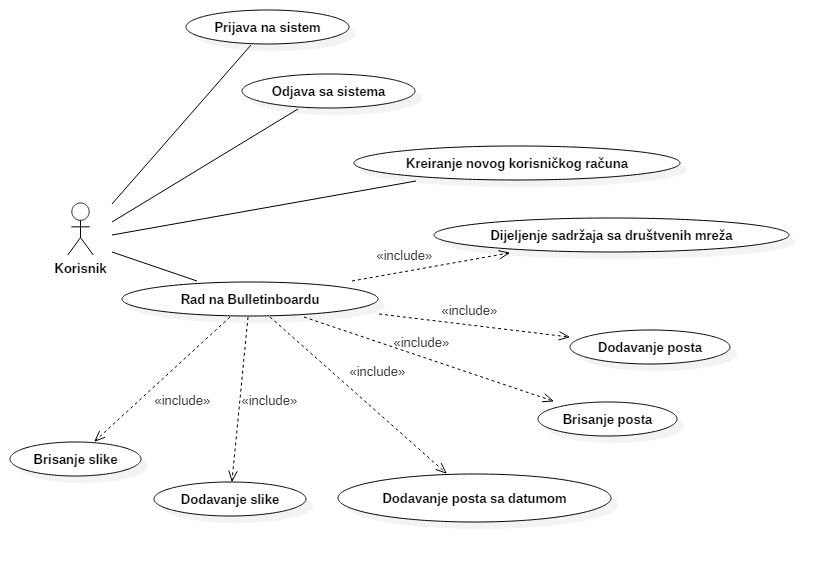
\includegraphics[scale=0.5]{SRS/use_cases/korisnik_use_case.png}

\subsubsection{Mogućnosti administratora}
Administrator sistema ima sljedeće mogućnosti:
\begin{itemize}
    \item Brisanje korisnika
    \item Pretraga i pregled korisnika
    \item Modifikacija korisnikovog profila
    \item Zabrana pristupa korisniku (ban)
    \item Održavanje sistema i korekcija grešaka
    \item Kreiranje izvještaja
    \item Pregled pinova koji imaju najveci broj djeljenja na mrežama
\end{itemize}
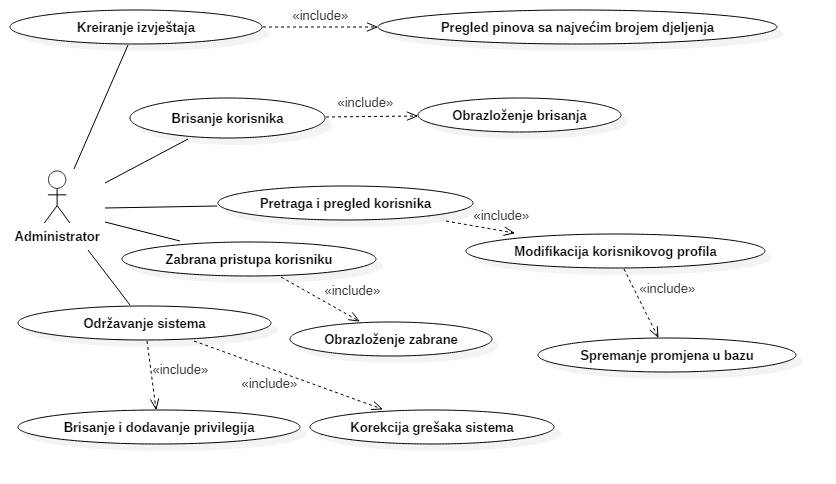
\includegraphics[scale=0.5]{SRS/use_cases/admin.png}
\subsection{Ograničenja}
\subsubsection{Zakonska ograničenja}
Zakonska ograničenja za ovaj sistem ne postoje. Postovi ne dozvoljavaju dijeljenje datoteka ili medijskog sadržaja, tako da sistem ne podliježe pravilnicima o zaštiti autorskih prava. Društvene mreže sa kojih je moguće dijeliti sadržaj u svojim pravima korištenja dozvoljavaju dijeljenje sadržaja, tako da tu ne postoje zabrane na koje je potrebno obratiti pažnju. U skladu sa navedenim, zaključuje se kako lokacija aplikacije nije ograničena lokalnim zakonima.
\subsubsection{Hardverska ograničenja}
Korisnički računari nemaju hardverska ograničenja. Potrebno je posjedovanje dovoljne konfiguracije za pokretanje web preglednika koji podržava novije internet protokole.

Za instalaciju servera i baze podataka koristit će se centralni računar sa minimalnom konfiguracijom:

\begin{itemize}
    \item Radna frekvencija procesora (CPU): 2.40GHz
    \item Količina RAM memorije: 4GB
    \item Količina memorije za trajno skladištenje (HDD): 500 GB
\end{itemize}

Po dogovoru sa klijentom, usluga se iznajmljuje od Cloud Operatera. Prilikom sklapanja ugovora sa pružaocem usluge Cloud Hostinga, preporučuje se konfiguracija virtualne mašine kakva je predviđena iznad ili bolja.

Za uspostavljanje izlaza na internet koristi će se mrežni kablovi, te sljedeći mrežni uređaji:
\begin{itemize}
  \item Switch: 10/100/1000 Mbps
  \item Ruter: 10/100 Mbps
\end{itemize}

Bitno je napomenuti kako konekciju na internet održava ISP i potrebna je stalna internet konekcija za pristup aplikaciji.
\subsubsection{Softverska ograničenja}
Korisnici aplikaciji mogu pristupiti putem jednog od sljedećih internet pretraživača: Firefox 52+, Chrome, Microsoft Edge.

Na serverskoj strani je potrebno obezbijediti MongoDB bazu podataka te operativni sistem sa instaliranim JRE (Java SE Runtime Environment) 8, ili novijim.

\subsection{Pretpostavke i zavisnosti}
\begin{itemize}
    \item \textbf{Pretpostavka 1.} Pretpostavlja se da se radi na novom informacionom sistemu, a ne na nadogradnji postojećeg. Nije potrebno raditi integraciju sa postojećim komponentama i prilagođavati se postojećem sistemu.
    \item \textbf{Pretpostavka 2.} Pretpostavlja se da je moguće nabaviti hardverske resurse potrebne za održavanje stranice aktivnom. Preporučeno je da se te usluge iznamljuju od cloud providera putem virtuelnih mašina.
    \item \textbf{Pretpostavka 3.} Pretpostavlja se da hardver ima instaliran potreban softver naveden u poglavlju "Softverski zahtjevi". Neki dijelovi softvera imaju licence za slobodno korištenje, dok je za druge potrebno platiti korištenje.
    \item \textbf{Pretpostavka 4.} Pretpostavlja se da serverski računari imaju svu potrebnu fizičku zaštitu. Ukoliko se koristi hardver cloud providera takvi uslovi se podrazumijevaju sklapanjem ugovora sa pružaocem usluge. Ukoliko se koristi vlastiti hardver, potrebno je osigurati dovoljan nivo zaštite da se server i rad sistema ne dovede u opasnost.
    \item \textbf{Pretpostavka 5.} Pretpostavlja se da serverski računar ima obezbijeđeno stabilno napajanje u svakom trenutku (24h dnevno). Prilikom sklapanja ugovora sa pružaocem cloud hosting usluge, dogovara se procenat vremena u kojem je usluga dostupna. Ukoliko se koristi vlastiti hardver, potrebno je osigurati UPS uređaje koji pružaju mogućnost napajanja u kriznim situacijama, kako bi sistem mogao nesmetano raditi.
    \item \textbf{Pretpostavka 6.} Preetpostavlja se da korisnici sistema imaju dovoljne hardverske konfiguracije za pristupanje web aplikaciji.
    \item \textbf{Pretpostavka 7.} Pretpostavlja se da korisnici sistema posjeduju osnovno poznavanje rada na računaru, pristupa i korištenja interneta.
    \item \textbf{Pretpostavka 8.} Pretpostavlja se da pristup serverskom računaru sa centralnom bazom podataka nema niko osim ovlaštene osobe, te da ovlaštena osoba neće zloupotrijebiti svoj položaj i vršiti manipulacije nad zapisima u bazi podataka. Ukoliko je sklopljen ugovor sa pružaocem cloud usluge, pretpostavlja se da će pružaoc poštovati stavke ugovora o čuvanju privatnosti i ograničenju neovlaštenog pristupa.
    \item \textbf{Pretpostavka 9.} Pretpostavlja se da ukoliko u toku ili nakon izrade sistema dođe do promjene zahtjeva ili dodatnih zahtjeva za funkcionalnostima, potrebno je pratiti korake koji su navedeni u poglavlju 2.6. Planiranje zahtjeva ovog dokumenta.
\end{itemize}
\subsection{Planiranje zahtjeva}
Kao početni dio razvoja softvera i cjelokupnog informacionog sistema, rade se faze analize zahtjeva i dizajna. Prvenstveno se radi analiza funkcionalnih i nefunkcionalnih zahtjeva, kao i navedenih ograničenja (zakonskih, hardverskih, softverskih). U slučaju eventualnih promjena zahtjeva potrebno je pratiti ustaljenu proceduru opisanu sljedećim koracima:
\begin{itemize}
    \item Od naručioca sistema se zahtjeva da dostavi zvanični zahtjev za promjenu funkcionalnosti sa detaljno opisanim traženim funkcionalnostima i promjenama nad sistemom.
    \item SI Pinboard Team se obavezuje da će u najkraćem roku od prijema zahtjeva uraditi analizu traženih promjena i dostaviti odgovor u vidu ponude koja opisuje mogućnost izvedbe traženih funkcionalnosti.
    \item Ukoliko je ponuda prihvatljiva, SRS se revidira i postaje nova, važeća, verzija dokumenta.
\end{itemize}

U slučaju da dođe do promjene zahtjeva nakon zaključivanja specifikacije, razvojni tim zadržava pravo na ne izvršavanje traženih promjena.

U slučaju da razvojni tim ima prijedlog na postojeće funkcionalnosti sistema nakon zaključivanja specifikacije, potrebno je pratiti ustaljenu proceduru opisanu sljedećim koracima:
\begin{itemize}
    \item Od razvojnog tima se zahtjeva da dostavi zvaničnu promjenu funkcionalnosti sa detaljno opisanim traženim funckcionalnostima i promjenama nad sistemom uključujući i utjecaj koji promjene imaju na vrijeme i cijenu razvoja.
    \item Naručilac sistema je dužan u roku 15 dana donijeti zaključak o predloženim izmjenama.
    \item Ukoliko je ponuda prihvatljiva, SRS se revidira i postaje nova, važeća, verzija dokumenta.
\end{itemize}

\newpage
\section{Konkretni zahtjevi}
\subsection{Vanjski interfejsi}
Interferjs omogućava komunikaciju sistema sa vanjskim ulazom/izlazom. To može da bude korisnik ili neki drugi sistem. Poštujući principe razvoja softvera, interfejs ne otkriva unutrašnju strukturu sistema već samo služi za razmjenu informacija.
\subsubsection{Korisnički interfejs}
Obzirom da su svi korisnici sistema podjednaki, nije potrebno implementirati sistem permisija. Razlikovanje među korisnicima se vrši na osnovu njihovih pristupnih podataka. Svaki korisnik ima pristup svom sadržaju.

Komunikacija sa korisnikom se radi na intuitivan način. Kako bi se izvršilo diferenciranje između drugih dijelova sistema, koriste se lako uočljive promjene u boji. Kontrast boje fonta u odnosu na podlogu omogućava laku uočljivost poruka. Tooltipovi daju savjete za korištenje funkcionalnosti sistema i sadrže osnovne informacije vezane za dati kontekst.

Sve funkcionalnosti korisničkog interfejsa upućene su ka lakšem dodavanju i pregledu sadržaja, kao i lakom uklanjanju i modifikaciji postojećeg sadržaja.

\subsubsection{Vanjski interfejsi}
Omogućena je komunkacija sa vanjskim sistemima, prvenstveno društvenim mrežama. Na taj način se korisniku daje mogućnost dijeljenja sadržaja sa društvenih mreža Instagram i Facebook na svoj profil unutar sistema. Omogućeno je i dijeljenje sadržaja sa sistema na druge platforme.

Komunikacija sa društvenim mrežama se odvija putem standardizovanog API-ja koji nudi data društvena mreža (Facebook, Instagram, Google).
\newpage
\subsection{Funkcionalni zahtjevi}

\subsubsection{Kreiranje novog korisničkog računa}
\begin{tabu} to 1.2\textwidth {p{4cm}p{8cm}}
 Opis: & Sistem pruža korisniku opciju kreiranja novog korisničkog računa kojim će se istom korisniku omogućiti pristup personalnom Bulletin boardu\\
Preduslovi: & Korisnik ima internet konekciju i validnu ličnu email adresu ili račun na nekoj od stranica: Instagram, Google, Facebook.\\
Ulaz: & Email adresa i password \\
Uslovi validnosti: & Postojeća email adresa \\
Procesiranje: & Korisnik unosi svoje podatke i sistem ih validira, te kreira korisnički račun povezan sa unesenom email adresom, nakon čega se pristupa Bulletin boardu \\
Izlaz: & Kreiran korisnički račun \\
Funkcionalni zahtjevi: & Sistem omogućava kreiranje novog korisničkog računa \\
Prioritet realizacije: & 1

\end{tabu}
\newpage
\subsubsection{Prijava na sistem}
\begin{tabu} to 1.2\textwidth {p{4cm}p{8cm}}
 Opis: & Korisnik se prijavljuje na sistem koristeći već kreiran korisnički račun i pristupa svom Bulletin boardu koji kasnije može uređivati\\
Preduslovi: & Korisnik ima kreiran korisnički račun \\
Ulaz: & Podaci potrebni za izvršenje prijave (email i password) ili prijava na povezani Google, Instagram ili Facebook račun \\
Uslovi validnosti: & Ispravno uneseni podaci (ili postojeći korisnički račun sa društvenih mreža) \\
Procesiranje: & Korisnik unosi svoje podatke u predviđena polja te ih sistem validira u svrhu omogućavanja pristupa korisničkom boardu ili ispisa greške ako podaci nisu validni\\
Izlaz: & Otvara se korisnikova početna stranica (Bulletin board) sa kojom on nastavlja daljnji rad (uređivanje) \\
Funkcionalni zahtjevi: & Sistem omogućava: Prijava na sistem, otvaranje sesije - sistem nudi sigurnost na ovaj način. \\
Prioritet realizacije & 1 \\
\end{tabu}
\newpage
\subsubsection{Odjava sa sistema}

\begin{tabu} to 1.2\textwidth {p{4cm}p{8cm}}
 Opis: & Korisnik se odjavljuje sa sistema i gubi pristup svom Bulletin boardu dok se ne prijavi opet \\
Preduslovi: & Korisnik je prethodno već prijavljen na sistem \\
Ulaz: & Odabir opcije za odjavu sa sistema \\
Uslovi validnosti: & - \\
Procesiranje: & Korisnik bira opciju odjave, sistem je procesira i odjavljuje korisnika sa sistema, onemogućavajući daljnji rad na boardu \\
Izlaz:& Korisnik je preusmjeren na login stranicu \\
Funkcionalni zahtjevi: & Sistem omogućava odjavu \\
Prioritet realizacije: & 1

\end{tabu}
\newpage


\subsubsection{Brisanje korisničkog računa}

\begin{tabu} to 1.2\textwidth {p{4cm}p{8cm}}
Opis: & Korisnik ima mogućnost da izbriše svoj profil u slučaju kada više ne želi koristiti aplikaciju. \\
Preduslovi: & Korisnik je prijavljen na sistem. \\
Ulaz: & Forma/Dijalog konfirmacije (Da li ste sigurni da želite obrisati profil? ) \\
Uslovi validnosti: & Korisnik mora imati profil na sistemu, ali svakako neće biti u mogućnosti da pristupi ruti za brisanje računa u slučaju da nije logovan na sistem \\
Procesiranje: & Kada korisnik klikne na opciju izbriši profil aktivira se konfirmacijski prozor u kojem korisnik ima dvije opcije Da/Ne. U slučaju da korisnik klikne na opciju “DA” modifikujemo u bazi kolonu “izbrisan” tj. Postavljamo je na true. Nakon promjene u bazi korisniku se prikazuje povratna poruka da mu je profil izbrisan i onda  prozor za prijavu/registraciju. \\
Izlaz: & Povratna poruka da je korisnikov profil izbrisan. \\
Funkcionalni zahtjevi: & Sistem omogućava: Brisanje profila \\
Prioritet realizacije: & 1

\end{tabu}
\newpage
\subsubsection{Modifikacija korisničkog računa}

\begin{tabu} to 1.2\textwidth {p{4cm}p{8cm}}
 Opis: & Korisnik ima mogućnost da mjenja podatke koje je prilikom registracije izabrao. \\
Preduslovi: & Korisnik je prijavljen na sistem. \\
Ulaz: & Forma/Dijalog update-a podataka koji sadrži labele i inpute ispunjene unesenim podacima prikom registracije. \\
Uslovi validnosti: & Korisnik mora imati profil na sistemu. Novi inputi moraju biti validirani. (Email mora biti u obliku email adrese) \\
Procesiranje: & Aplikacija otvara formu za uređivanje sa labelema i inputima ispunjenima sa unesenim podacima prilikom registracije. Korisnik upisuje nove podatke, pri čemu se inputi validiraju. Kada je korisnika zadovoljan sa novo unesenim podacima klikom na dugme Save, modifikuje se red u tabeli korisnika. \\
Izlaz: & Pregled pinboarda sa promjenjenim podacima. \\
Funkcionalni zahtjevi: & Sistem omogućava: Modifikacija korisničkog računa i validaciju novo unesenih podataka. \\
Prioritet realizacije: & 2

\end{tabu}
\newpage
\subsubsection{Dodavanje slike}

\begin{tabu} to 1.2\textwidth {p{4cm}p{8cm}}
 Opis: & Korisnik sistema bira sliku koju želi da postavi na svoj Bulletin board i uz nju piše željeni opis\\
Preduslovi: & Kreiran korisnički račun \\
Ulaz: & Slika (obavezno) i željeni opis (opcionalno) \\
Uslovi validnosti: & Izvršen download željene slike, te odabrana opcija za dodavanje slika \\
Procesiranje: & Korisnik vrši izbor slike koju želi da postavi na svoj personalizirani board te, po želji, dodaje opis uz istu \\
Izlaz: & Prikaz postavljene slike zajedno sa opisom \\
Funkcionalni zahtjevi: & Sistem omogućava: odabir slike, unos opisa, prekid opcije postavljanja, pregled postavljene slike \\
Prioritet realizacije: & 2

\end{tabu}
\newpage
\subsubsection{Okretanje (rotiranje) slike}

\begin{tabu} to 1.2\textwidth {p{4cm}p{8cm}}
 Opis: & Korisnik sistema bira sliku koju je prethodno postavio i okreće je u željenoj direkciji\\
Preduslovi: & Kreiran korisnički račun \\
Ulaz: & Slika koja je prehodno postavljena \\
Uslovi validnosti: & Odabrana opcija za rotiranje slike \\
Procesiranje: & Korisnik vrši izbor slike koju želi da rotira \\
Izlaz: & Prikaz rotirane slike zajedno sa opisom \\
Funkcionalni zahtjevi: & Sistem omogućava: odabir slike, rotiranje iste, pregled rotirane slike \\
Prioritet realizacije: & 2

\end{tabu}
\newpage
\subsubsection{Brisanje slike}

\begin{tabu} to 1.2\textwidth {p{4cm}p{8cm}}
Opis: & Korisnik sistema briše sliku koju je prethodno dodao i samim tim je uklanja sa sadržaja svog boarda \\
Preduslovi: & Korisnik je prijavljen sa sistem i prethodno je postavio sliku \\
Ulaz: & Slika koju je potrebno brisati \\
Uslovi validnosti: & Slika je označena \\
Procesiranje: & Korisnik selektuje sliku koju želi ukloniti (izbrisati) sa sadržaja svog boarda, te sistem istu briše uz prikazivanje poruke validacije u svrhu obavještavanja da li je zahtjev ispunjen ili nije \\
Izlaz: & Poruka o uspješnom brisanju slike \\
Funkcionalni zahtjevi: & Sistem omogućava: prikaz svih postavljenih slika, selektovanje slike koju korisnik želi brisati, brisanje slike iz sistema, prikaz poruke o uspješnom brisanju \\
Prioritet realizacije: & 2

\end{tabu}
\newpage
\subsubsection{Dodavanje posta}

\begin{tabu} to 1.2\textwidth {p{4cm}p{8cm}}
Opis: & Sistem omogućava korisniku dodavanje novih personaliziranih postova na Bulletin board \\
Preduslovi: & Korisnik je prijavljen na sistem, te je odabrana opcija za dodavanje postova \\
Ulaz: & Željeni tekst \\
Uslovi validnosti: &  Odabrana opcija za dodavanje posta \\
Procesiranje: & Korisnik bira opciju za dodavanje posta, unosi željeni tekst, nakon čega je post vidljiv i dodan na board \\
Izlaz: & Prikaz dodanog posta na Bulletin boardu \\
Funkcionalni zahtjevi: & Sistem omogućava: dodavanje posta, prikaz posta na glavnom ekranu aplikacije, mogućnost manipulisanja dodanim postom \\
Prioritet realizacije: & 2

\end{tabu}
\newpage
\subsubsection{Brisanje posta}

\begin{tabu} to 1.2\textwidth {p{4cm}p{8cm}}
Opis: & Korisnik sistema uklanja (odnosno briše) post koji je prethodno dodao na svoj board\\
Preduslovi: & Korisnik je prijavljen sa sistem i prethodno je dodao post \\
Ulaz: & Post koji je potrebno brisati \\
Uslovi validnosti: & Post je označen \\
Procesiranje: & Korisnik selektuje post koji želi brisati, te sistem isti briše \\
Izlaz: & Poruka o uspješnom brisanju posta \\
Funkcionalni zahtjevi: & Sistem omogućava: prikaz svih dodanih postova, selektovanje posta koji korisnik želi brisati, brisanje posta iz sistema, prikaz poruke o uspješnom brisanju \\
Prioritet realizacije: & 2

\end{tabu}
\newpage
\subsubsection{Sakrivanje posta}

\begin{tabu} to 1.2\textwidth {p{4cm}p{8cm}}
Opis: & Korisnik sistema sakriva ali i ne uklanja trajno post koji je prethodno dodao na svoj board\\
Preduslovi: & Korisnik je prijavljen sa sistem i prethodno je dodao post koji sada želi sakriti \\
Ulaz: & Post koji je potrebno sakriti \\
Uslovi validnosti: & Post je označen \\
Procesiranje: & Korisnik selektuje post koji želi sakriti, te sistem isti sakriva \\
Izlaz: & \\
Funkcionalni zahtjevi: & Sistem omogućava: prikaz svih dodanih postova, selektovanje posta koji korisnik želi sakriti \\
Prioritet realizacije: & 2

\end{tabu}
\newpage
\subsubsection{Dodavanje posta sa datumom (kalendar)}

\begin{tabu} to 1.2\textwidth {p{4cm}p{8cm}}
Opis & Korisnik na svoj pinboard profil dodaje post sa postavljenim datumom \\
Preduslovi & Korisnik je prijavljen na sistem \\
Ulaz & Odabir datuma, boje posta i teksta vezanog za post  \\
Uslovi validnosti & / \\
Procesiranje & Bira se datum na kalendaru, unosi se tekst za post i post se spašava klikom na dugme spasi\\
Izlaz & Novi post sa datumom se dodaje na pinboard feed \\
Funkcionalni zahtjevi & Dodavanje posta, odabir datuma na kalendaru \\
Prioritet realizacije & 2 \\
\end{tabu}
\newpage
\subsubsection{Dijeljenje sadržaja sa društvenih mreža}


\begin{tabu} to 1.2\textwidth {p{4cm}p{8cm}}
Opis: & Korisnik sistema dijeli na pinboard sadržaj koji je prethodno postavljen na jednu od ponuđenih društvenih mreža \\
Preduslovi: & Korisnik ima kreiran korisnički račun na ponuđenim društvnenim mrežama \\
Ulaz: & Postojeći sadržaj na društvenim mrežama koji korisnik želi da podijeli \\
Uslovi validnosti: & Odabran sadržaj koji se želi podijeliti \\
Procesiranje: & Korisnik bira na društvenim mrežama sadržaj koji želi da podijeli na pinboard, te prolazi kroz dijalog dijeljenja u sistemu pinboarda pri čemu može da prihvati već postojeće postavke/opise, izmijeni ih ili odustane od samog procesa dijeljenja. \\
Izlaz: & Sadržaj podijeljen sa društvene mreže na pinboard
Funkcionalni zahtjevi: Sistem omogućava: povezivanje sa odabranom društvenom mrežom, dijeljenje sadržaja postavljenog na društvenoj mreži, preusmjeravanje na link originalnog posta na društvenoj mreži \\
Prioritet realizacije: & 3

\end{tabu}
\newpage
\newpage
\subsection{Nefunkcionalni zahtjevi i osobine sistema}
\subsubsection{Upotrebljivost sistema}
\begin{itemize}
    \item \textbf{NFZ 1.} Korisnički interfejs će biti napisan na bosanskom jeziku. Bit će intuitivan i nedvosmislen, ujedno i jednostavan za shvatiti.
    \item \textbf{NFZ 2.} Slične opcije će biti implementirane tako da imaju sličnu sekvencu akcija.
    \item \textbf{NFZ 3.} Bit će omogućene poruke o nastalim greškama, koje će se odmah prikazivati u slučaju da dođe do greške.
    \item \textbf{NFZ 4.} Dugme za pomoć će biti lako uočljivo i omogućit će korisniku upute za korištenje.
\end{itemize}

\subsubsection{Performanse sistema}
\begin{itemize}
    \item \textbf{NFZ 5.} Performanse sistema zavise od cloud provajdera.
    \item \textbf{NFZ 6.} Nivoi usluga će biti definisani SLA ugovorom.
\end{itemize}

\subsection{Atributi kvalitete sistema}
\subsubsection{Fizička sigurnost}
    \begin{itemize}
        \item \textbf{NFZ 7.} S obzirom da će aplikacija biti hostovana na cloud server fizička sigurnost se oslanja na kvalitet fizičke sigurnosti podatkovnih centara. To garantuje dobru redudantnu povezivost, redudantno električno napajanje, fizičku sigurnost zgrade, zamjenu pokvarenih uređaja, protupožarni sistem, sistem za hlađenje, te autorizaciju osoblja.
    \end{itemize}
\subsubsection{Sigurnost}
    \begin{itemize}
        \item \textbf{NFZ 8.} Korisniku će biti omogućene samo one funkcionalnosti za koje ima pravo pristupa.
        \item \textbf{NFZ 9.} Ukoliko podaci prilikom registracije ili prijave budu neispravni korisnik će biti upozoren.
        \item \textbf{NFZ 10.} Lozinka nije automatski dodijeljena, već je korisnik sam izabrao.
        \item \textbf{NFZ 11.} Lozinke moraju biti duge minimalno 7 karaktera (sastoje se od slova engleskog alfabeta i bar jedne cifre).
        \item \textbf{NFZ 12.} Budući da se radi o cloudu podaci trebaju biti kriptovani.
    \end{itemize}
\subsubsection{Backup}
\begin{itemize}
    \item \textbf{NFZ 13.} Vršit će se automatski backup podataka na cloud.
\end{itemize}
\subsubsection{Portabilnost}
\begin{itemize}
    \item \textbf{NFZ 14.} Bit će omogućeno korištenje na svim operativnim sistemima uz pretpostavku da postoji internet konekcija. 
\end{itemize}
\subsubsection{Skalabilnost}
\begin{itemize}
    \item \textbf{NFZ 15.} Dobro dizajnirana aplikacija će omogućiti lako uvođenje novih funkcionalnosti ukoliko se za istim ukaže potreba. 
\end{itemize}
\subsubsection{Dostupnost}
\begin{itemize}
    \item \textbf{NFZ 16.} U slučaju nestanka internet konekcije korisnik ne može pristupiti aplikaciji
    \item \textbf{NFZ 17.} Svevremenski dostupna aplikacija osim u slučaju nepredviđenih situacija.
    \end{itemize}
\subsubsection{Održavanje}
\begin{itemize}
    \item \textbf{NFZ 18.} Uslovi održavanja aplikacije se dogovaraju sa klijentom u predstojećim dokumentima. Nadogradnja se radi na osnovu dogovorenog procesa pri čemu su moguća vremena nedostupnosti aplikacije.
\end{itemize}

\newpage
\section{Korisnički Interfejs}

\subsection{Registracija}
Ekran koji dočekuje sve korisnike sistema pri samom pristupanju je pogled za Registraciju. Sadrži polja za unost teksta kako bi bilo moguće izvršiti registraciju novog korisnika u sistem. Korisnici koji su već dodani u sistem mogu pristupe pogledu za prijavu putem linka u dnu ekrana.


\centerline{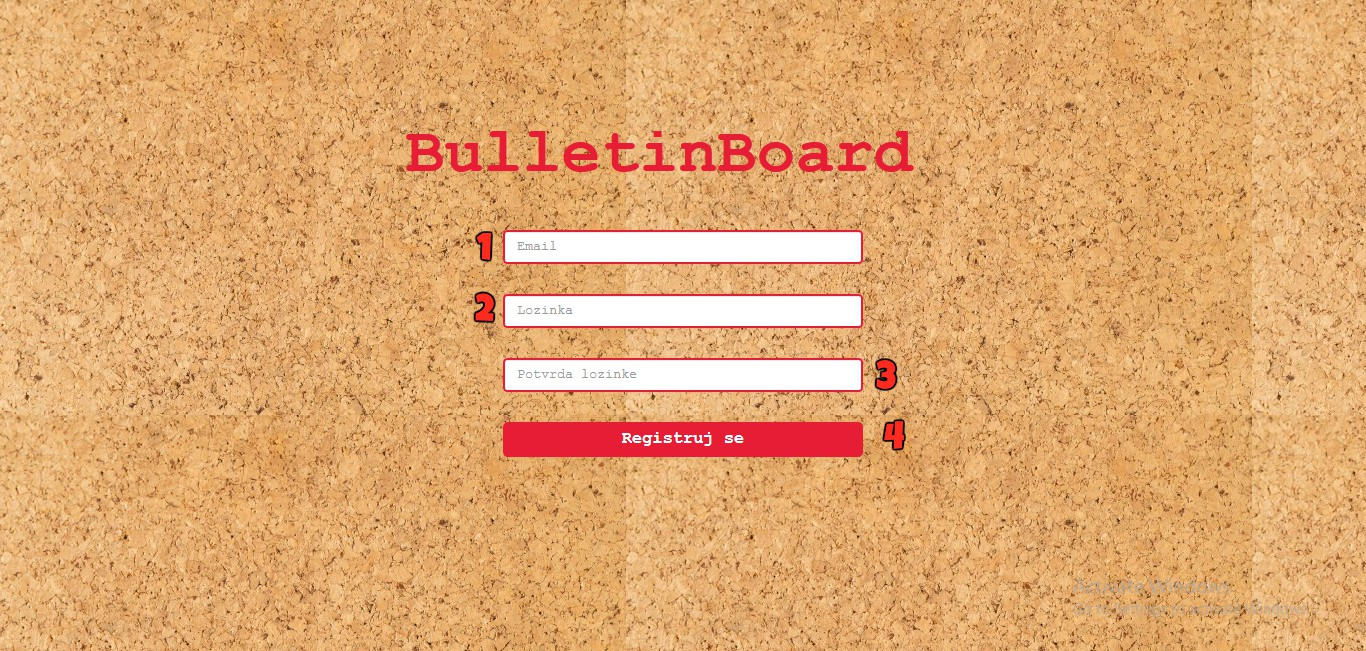
\includegraphics[scale=0.5]{slike/registracija_no.jpg}}
\begin{enumerate}
    \item Tekstualno polje u koje se unosi email za korisnički račun
    \item Tekstualno polje u koje se unosi password za korisnički račun
    \item Tekstualno polje u koje se unosi potvrda passworda za korisnički račun kako ne bi došlo do greške
    \item Dugme kojim se potvrđuje akcija registracije korisničkog računa
\end{enumerate}


\newpage

\subsection{Login}
Korisnici koji su se već registrovali u sistem trebaju se prijaviti prilikom svakog korištenja aplikacije. Na pogledu za prijavu se nalaze polja za unos teksta kako bi se unijeli username i password. Klikom na prijavu se vrši provjera i prijava na sistem.


\centerline{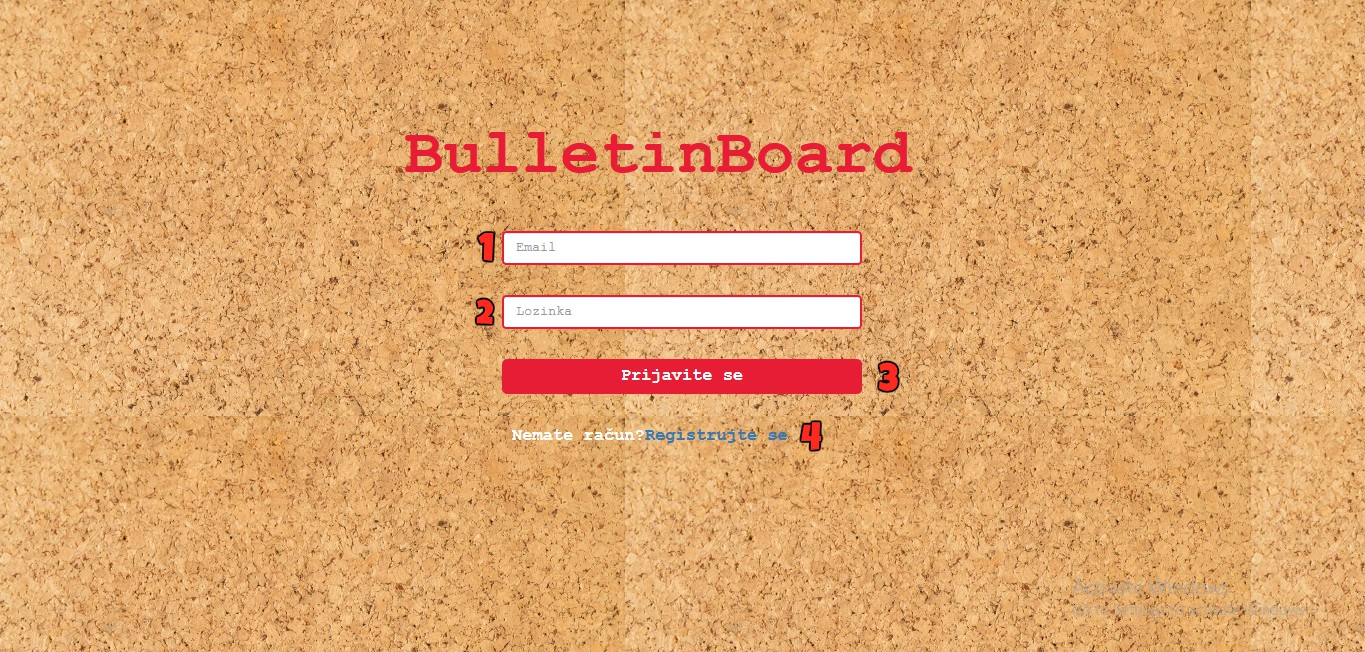
\includegraphics[scale=0.5]{slike/login_no.jpg}}
\begin{enumerate}
    \item Tekstualno polje u koje se unosi email za prijavu u korisnički račun
    \item Tekstualno polje u koje se unosi password za korisnički račun
    \item Dugme kojim se potvrđuje akcija prijave korisnika u sistem
    \item Link za pogled registracije novog korisničkog računa
\end{enumerate}

\newpage

\subsection{Dashboard}
Glavne funkcionalnosti aplikacije se izvršavaju na dashboard pogledu. Korisnici imaju mogućnosti za dodavanje zabilješki, brisanje i modifikaciju istih.


\centerline{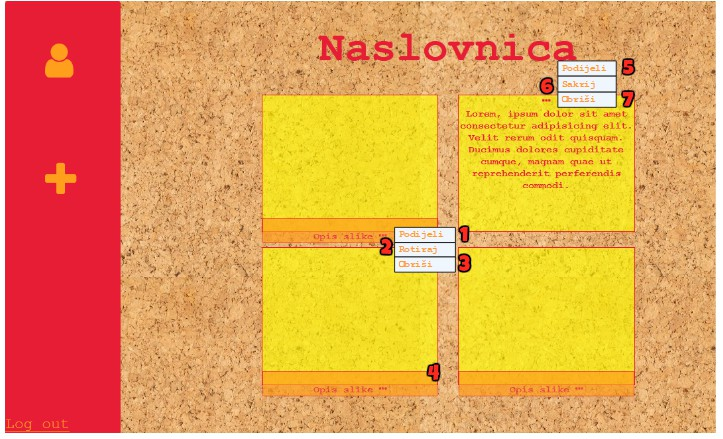
\includegraphics[scale=0.5]{slike/dash_no.jpg}}
\begin{enumerate}
    \item Opcija za dijeljenje slike 
    \item Opcija rotiranja slike
    \item Opcija izbriši sliku
    \item Textarea za dodavanje opisa slike
    \item Opcija za dijeljenje posta
    \item Opcija sakrivanja posta
    \item Opcija izbriši post
\end{enumerate}

\newpage


\subsection{Postavke}
Postavke korisnčkog računa moguće je mijenjati na pogledu za Postavke. Neki od korisničkih podataka koji se mogu mijenjati su prikazani na slici ispod.


\centerline{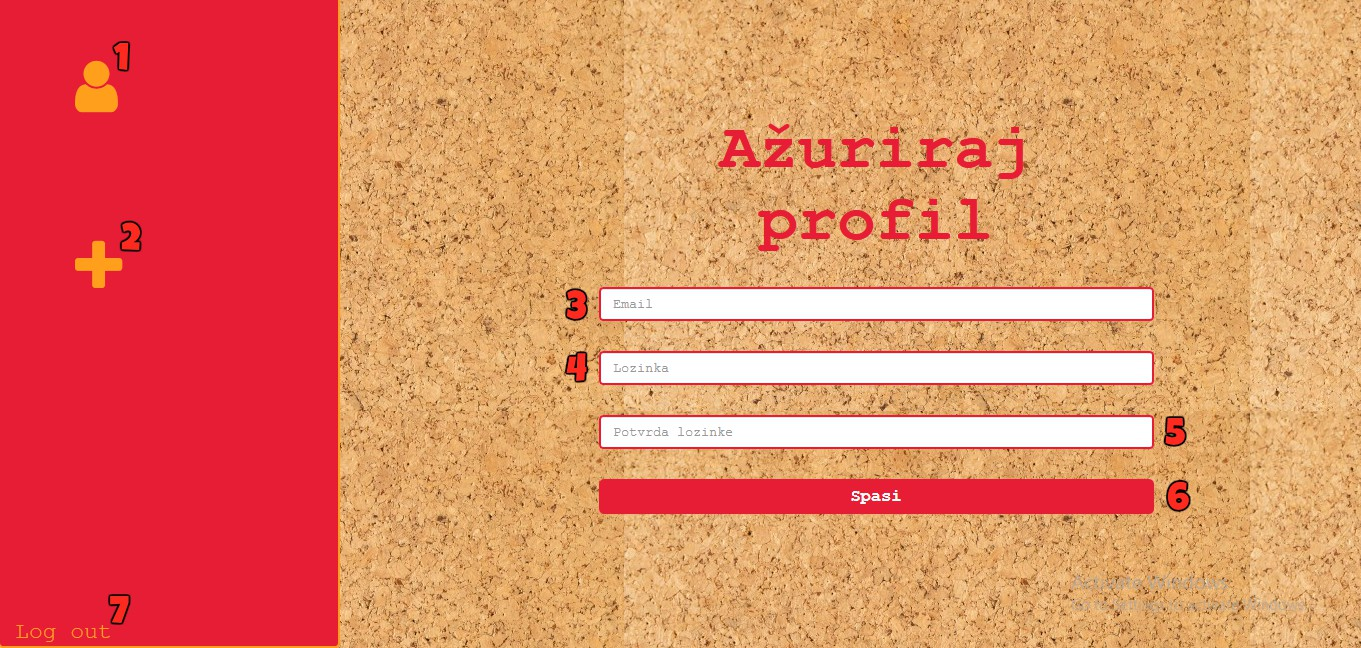
\includegraphics[scale=0.5]{slike/postavke_np.jpg}}
\begin{enumerate}
    \item Dugme koje vodi na korisnički račun
    \item Dugme za dodavanje nove zabilješke
    \item Tekstualno polje u koje se unosi email koji se mijenja
    \item Tekstualno polje u koje se unosi password za korisnički račun
    \item Tekstualno polje za unos potvrde passworda za korisnički račun
    \item Dugme kojim se potvrđuje akcija spašavanja novih postavki korisnika u sistemu
    \item Dugme za odjavljivanje prijavljenog korisnika iz sistema
\end{enumerate}




\end{document}
